% Standalone figure: TASLP Fig. 1, accept/defer reliability gate (G1 protocol).
% One protocol, two phases: offline speaker-disjoint calibration (top) freezes
% lambda^* via LTT + EB p-values + Bonferroni-over-grid; inference (bottom)
% reads decode artifacts from a frozen ASR backbone (never the model) to a
% confidence s. Both phases meet at the hinge s >= lambda^*; accept carries the
% macro-CER <= alpha w.p. >= 1-delta guarantee, else defer to a human. If no
% lambda on the grid certifies, the calibration fork reports VACUOUS-AT-TARGET
% (nothing accepted, not silently dropped). Not a 5-stage RISC schematic.
% Notation matches Methods (G1): s, lambda, lambda^*, n_cal, alpha, delta.
% No numeric values; no tool-name slogan in the rendered figure.
% Native width ~8.85cm so 8pt titles / 7.5pt subs stay at TASLP columnwidth.
% Compile: pdflatex fig0_overview.tex; Makefile copies PDF to ../figures and
% ../taslp/figures.
\documentclass[border=0.8pt]{standalone}
\usepackage[T1]{fontenc}
\usepackage{lmodern}
\usepackage{tikz}
\usepackage{amsmath,amssymb}
\usetikzlibrary{arrows.meta,positioning,fit,calc,backgrounds}

\definecolor{cAccept}{HTML}{0072B2}
\definecolor{cDefer}{HTML}{D55E00}
\definecolor{cVac}{HTML}{8A6D1A}
\definecolor{cBoxFill}{HTML}{F7F7F7}
\definecolor{cBoxLine}{HTML}{2F2F2F}
\definecolor{cCalFill}{HTML}{D9E6F2}
\definecolor{cInfFill}{HTML}{EFE6D8}
\definecolor{cGuardFill}{HTML}{D2E4F2}
\definecolor{cDeferFill}{HTML}{F3DFCC}
\definecolor{cVacFill}{HTML}{F2E9C4}
\definecolor{cHingeFill}{HTML}{FFFFFF}
\definecolor{cFrame}{HTML}{AFAFAF}

\newcommand{\sub}[1]{{\fontsize{7.5}{8.4}\selectfont #1}}
\newcommand{\ph}[1]{{\fontsize{7}{8}\selectfont #1}}

\begin{document}
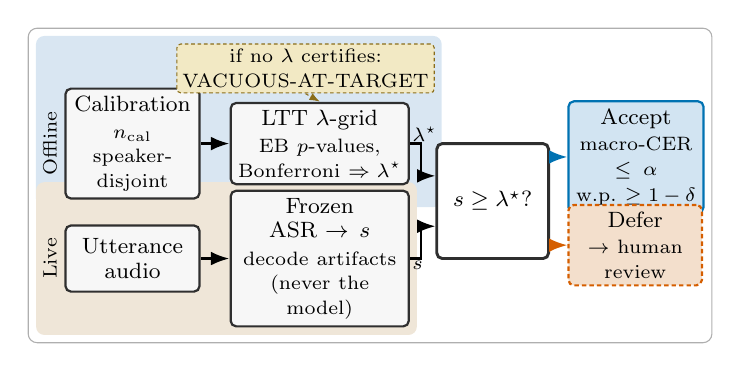
\begin{tikzpicture}[
  >=Latex,
  font=\fontsize{8}{9}\selectfont,
  pipebox/.style={
    draw=cBoxLine, thick, rounded corners=2pt, fill=cBoxFill,
    align=center, inner sep=2.6pt, minimum height=0.84cm, outer sep=0.5pt,
  },
  hingebox/.style={
    draw=cBoxLine, line width=1.05pt, rounded corners=2pt, fill=cHingeFill,
    align=center, inner sep=2.8pt, minimum width=1.42cm, minimum height=1.46cm,
    outer sep=0.5pt,
  },
  acceptbox/.style={
    draw=cAccept, thick, rounded corners=2pt, fill=cGuardFill,
    align=center, inner sep=2.8pt, minimum height=0.78cm, outer sep=0.4pt,
  },
  deferbox/.style={
    draw=cDefer, thick, dash pattern=on 1.6pt off 1.1pt, rounded corners=2pt,
    fill=cDeferFill, align=center, inner sep=2.5pt, minimum height=0.70cm,
    outer sep=0.4pt,
  },
  vacbox/.style={
    draw=cVac, thin, dash pattern=on 1.3pt off 1.0pt, rounded corners=1.4pt,
    fill=cVacFill, align=center, inner sep=2.0pt, outer sep=0.3pt,
  },
]

% Rotated swimlane labels (compact width; caption names calibration vs inference).
\node[rotate=90, inner sep=0pt, font=\fontsize{7}{8}\selectfont] (laboff)
  at (0.18, 1.46) {Offline};
\node[rotate=90, inner sep=0pt, font=\fontsize{7}{8}\selectfont] (lablive)
  at (0.18, 0.00) {Live};

% --- offline (top) ---
\node[pipebox, text width=1.52cm, anchor=west] (calsplit) at (0.36, 1.46)
  {Calibration\\[0.8pt]\sub{$n_{\mathrm{cal}}$}\\[-0.2pt]\sub{speaker-disjoint}};
\node[pipebox, text width=2.08cm, anchor=west, right=0.36cm of calsplit] (ltt)
  {LTT $\lambda$-grid\\[0.8pt]\sub{EB $p$-values,}\\[-0.2pt]\sub{Bonferroni $\Rightarrow\lambda^\star$}};

% --- live inference (bottom) ---
\node[pipebox, text width=1.52cm, anchor=west] (utt) at (0.36, 0.00)
  {Utterance audio};
\node[pipebox, text width=2.08cm, anchor=west, right=0.36cm of utt] (backbone)
  {Frozen ASR $\to s$\\[0.8pt]\sub{decode artifacts}\\[-0.2pt]\sub{(never the model)}};

% Vacuous fork: two lines, same width as LTT (must not widen the figure).
\node[vacbox, above=0.10cm of ltt, xshift=-0.18cm] (vac)
  {\sub{if no $\lambda$ certifies:}\\[-0.2pt]\fontsize{6.8}{7.8}\selectfont VACUOUS-AT-TARGET};

% Hinge: one-line comparison, vertically centered between the two phases.
\node[hingebox, anchor=west] (dec) at ($(ltt.east)+(0.32,-0.73)$)
  {\fontsize{8.5}{10}\selectfont $s\ge\lambda^\star$?};

% Outcomes to the right (keeps column height down; real gap, no chip overlap).
\node[acceptbox, text width=1.52cm, anchor=west]
  (guarantee) at ($(dec.east)+(0.22,0.56)$)
  {Accept\\[0.6pt]\sub{macro-CER $\le\alpha$}\\[0.2pt]\sub{w.p.\ $\ge 1-\delta$}};
\node[deferbox, text width=1.52cm, anchor=west]
  (defer) at ($(dec.east)+(0.22,-0.56)$)
  {Defer\\[0.5pt]\sub{$\to$ human review}};

\draw[->, thick] (calsplit) -- (ltt);
\draw[->, thick] (utt) -- (backbone);

\draw[->, thick] (ltt.east) -- ++(0.14,0) |- ($(dec.west)+(0,0.32)$);
\draw[->, thick] (backbone.east) -- ++(0.14,0) |- ($(dec.west)+(0,-0.32)$);
\node[anchor=south west, inner sep=0.3pt] at ($(ltt.east)+(0.01,0.01)$)
  {\sub{$\lambda^\star$}};
\node[anchor=north west, inner sep=0.3pt] at ($(backbone.east)+(0.01,-0.01)$)
  {\sub{$s$}};

\draw[->, thick, cAccept] (dec.east |- guarantee.west) -- (guarantee.west);
\draw[->, thick, cDefer, dash pattern=on 1.6pt off 1.1pt]
  (dec.east |- defer.west) -- (defer.west);
\draw[-{Latex[length=1.3mm]}, thin, cVac, dash pattern=on 1.2pt off 1.0pt]
  (vac.south) -- (ltt.north);

\begin{scope}[on background layer]
  \node[rounded corners=3pt, inner xsep=2.4pt, inner ysep=2.6pt,
        fill=cCalFill, fit=(laboff)(calsplit)(ltt)(vac)] (bandoff) {};
  \node[rounded corners=3pt, inner xsep=2.4pt, inner ysep=2.6pt,
        fill=cInfFill, fit=(lablive)(utt)(backbone)] (bandlive) {};
  \node[rounded corners=3.2pt, inner sep=2.6pt, draw=cFrame, thin,
        fit=(bandoff)(bandlive)(dec)(guarantee)(defer)] {};
\end{scope}

\end{tikzpicture}
\end{document}
